\section{Auswertung}
\label{sec:Auswertung}
\subsection{Photodetektorschaltung}
\label{subsec:PhotDet}
Es wurde die Schaltung wie in \autoref{} aufgebaut und die Messergebnisse aus \autoref{tab:DatenPhotoDet} in \autoref{fig:PhotoDet} in ein Diagramm eingetragen.
Außerdem sind die Daten an die Funktionen
\begin{align*}
    U &= \frac{a_1}{r} + b_1\\
    U &= \frac{a_2}{r^2} + b_2\\
\end{align*}
\\
gefittet worden. Bei diesen Ausgleichsrechnungen ergeben sich die Parameter zu
\begin{align*}
  a_1 &= 14.8304\pm 1.1554\\
  b_1 &= -53.1389\pm 10.1302\\
  a_2 &= 0.9299\pm 0.0264\\
  b_2 &= -9.1041\pm 2.6981\\
\end{align*}
Daraus folgt, dass sich die Funktion der Lichtintensität $\varpropto \frac{1}{r^2}$ verhält. Zudem wird \autoref{fig:PhotoDet}
entnommen, dass $r_{max}$ ca. zwischen $\SI{50}{\centi\meter}$ und $\SI{60}{\centi\meter}$ liegt, da die Kurve von dort an nicht mehr signifikant abfällt und nur noch
das Umgebungslicht gemessen wird, wordurch diese niemals gegen Null geht, sondern gegen einen konstanten Wert $>0$.
\begin{table}
  \centering
  \caption{Die gemessenen Spannungen zum zugehörigen Abstand der LED zum Photodetektor.}
  \begin{tabular}{cc}
    \toprule
    {$U \mathbin{/} \unit{\volt}$} &
    {$r \mathbin{/} \unit{\centi\meter}$} \\
    \midrule
      210.0 & 6.6 \\
      194.0 & 7.0 \\
      170.0 & 7.5 \\
      138.0 & 8.0 \\
      110.0 & 8.5 \\
      93.6 & 9.0 \\
      83.2 & 9.5 \\
      74.4 & 10.0 \\
      60.0 & 11.0 \\
      48.0 & 12.0 \\
      40.0 & 13.0 \\
      32.4 & 14.0 \\
      28.0 & 15.0 \\
      20.4 & 17.0 \\
      16.2 & 19.0 \\
      12.8 & 21.0 \\
      11.4 & 23.0 \\
      9.0 & 25.0 \\
      6.9 & 30.0 \\
      5.5 & 40.0 \\
      4.5 & 50.0 \\
      3.9 & 60.0 \\
    \bottomrule
  \end{tabular}
  \label{tab:DatenPhotoDet}
\end{table}
\begin{figure}
  \centering
  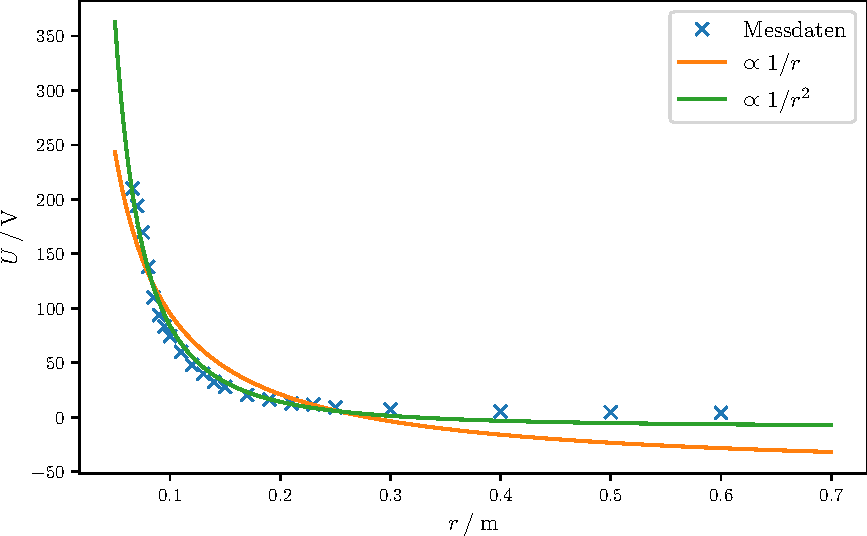
\includegraphics{Led-Messung.pdf}
  \caption{Die Messwerte aus \autoref{tab:DatenPhotoDet} und die Ausgleichsrechnungen in einem Diagramm aufgetragen.}
  \label{fig:PhotoDet}
\end{figure}
